


\documentclass[onecolumn, conference, 12pt]{IEEEtran}


% Some very useful LaTeX packages include:
% (uncomment the ones you want to load)


% *** MISC UTILITY PACKAGES ***
%
%\usepackage{ifpdf}
% Heiko Oberdiek's ifpdf.sty is very useful if you need conditional
% compilation based on whether the output is pdf or dvi.
% usage:
% \ifpdf
%   % pdf code
% \else
%   % dvi code
% \fi
% The latest version of ifpdf.sty can be obtained from:
% http://www.ctan.org/pkg/ifpdf
% Also, note that IEEEtran.cls V1.7 and later provides a builtin
% \ifCLASSINFOpdf conditional that works the same way.
% When switching from latex to pdflatex and vice-versa, the compiler may
% have to be run twice to clear warning/error messages.






% *** CITATION PACKAGES ***
%
\usepackage{cite}
% cite.sty was written by Donald Arseneau
% V1.6 and later of IEEEtran pre-defines the format of the cite.sty package
% \cite{} output to follow that of the IEEE. Loading the cite package will
% result in citation numbers being automatically sorted and properly
% "compressed/ranged". e.g., [1], [9], [2], [7], [5], [6] without using
% cite.sty will become [1], [2], [5]--[7], [9] using cite.sty. cite.sty's
% \cite will automatically add leading space, if needed. Use cite.sty's
% noadjust option (cite.sty V3.8 and later) if you want to turn this off
% such as if a citation ever needs to be enclosed in parenthesis.
% cite.sty is already installed on most LaTeX systems. Be sure and use
% version 5.0 (2009-03-20) and later if using hyperref.sty.
% The latest version can be obtained at:
% http://www.ctan.org/pkg/cite
% The documentation is contained in the cite.sty file itself.


% *** GRAPHICS RELATED PACKAGES ***
%
\ifCLASSINFOpdf
\usepackage[pdftex]{graphicx}
% declare the path(s) where your graphic files are
% \graphicspath{{../pdf/}{../jpeg/}}
% and their extensions so you won't have to specify these with
% every instance of \includegraphics
% \DeclareGraphicsExtensions{.pdf,.jpeg,.png}
\else
% or other class option (dvipsone, dvipdf, if not using dvips). graphicx
% will default to the driver specified in the system graphics.cfg if no
% driver is specified.
% \usepackage[dvips]{graphicx}
% declare the path(s) where your graphic files are
% \graphicspath{{../eps/}}
% and their extensions so you won't have to specify these with
% every instance of \includegraphics
% \DeclareGraphicsExtensions{.eps}
\fi
% graphicx was written by David Carlisle and Sebastian Rahtz. It is
% required if you want graphics, photos, etc. graphicx.sty is already
% installed on most LaTeX systems. The latest version and documentation
% can be obtained at: 
% http://www.ctan.org/pkg/graphicx
% Another good source of documentation is "Using Imported Graphics in
% LaTeX2e" by Keith Reckdahl which can be found at:
% http://www.ctan.org/pkg/epslatex
%
% latex, and pdflatex in dvi mode, support graphics in encapsulated
% postscript (.eps) format. pdflatex in pdf mode supports graphics
% in .pdf, .jpeg, .png and .mps (metapost) formats. Users should ensure
% that all non-photo figures use a vector format (.eps, .pdf, .mps) and
% not a bitmapped formats (.jpeg, .png). The IEEE frowns on bitmapped formats
% which can result in "jaggedy"/blurry rendering of lines and letters as
% well as large increases in file sizes.
%
% You can find documentation about the pdfTeX application at:
% http://www.tug.org/applications/pdftex





% *** MATH PACKAGES ***
%
\usepackage{amsmath}
% A popular package from the American Mathematical Society that provides
% many useful and powerful commands for dealing with mathematics.
%
% Note that the amsmath package sets \interdisplaylinepenalty to 10000
% thus preventing page breaks from occurring within multiline equations. Use:
\interdisplaylinepenalty=2500
% after loading amsmath to restore such page breaks as IEEEtran.cls normally
% does. amsmath.sty is already installed on most LaTeX systems. The latest
% version and documentation can be obtained at:
% http://www.ctan.org/pkg/amsmath





% *** SPECIALIZED LIST PACKAGES ***
%
%\usepackage{algorithmic}
% algorithmic.sty was written by Peter Williams and Rogerio Brito.
% This package provides an algorithmic environment fo describing algorithms.
% You can use the algorithmic environment in-text or within a figure
% environment to provide for a floating algorithm. Do NOT use the algorithm
% floating environment provided by algorithm.sty (by the same authors) or
% algorithm2e.sty (by Christophe Fiorio) as the IEEE does not use dedicated
% algorithm float types and packages that provide these will not provide
% correct IEEE style captions. The latest version and documentation of
% algorithmic.sty can be obtained at:
% http://www.ctan.org/pkg/algorithms
% Also of interest may be the (relatively newer and more customizable)
% algorithmicx.sty package by Szasz Janos:
% http://www.ctan.org/pkg/algorithmicx




% *** ALIGNMENT PACKAGES ***
%
%\usepackage{array}
% Frank Mittelbach's and David Carlisle's array.sty patches and improves
% the standard LaTeX2e array and tabular environments to provide better
% appearance and additional user controls. As the default LaTeX2e table
% generation code is lacking to the point of almost being broken with
% respect to the quality of the end results, all users are strongly
% advised to use an enhanced (at the very least that provided by array.sty)
% set of table tools. array.sty is already installed on most systems. The
% latest version and documentation can be obtained at:
% http://www.ctan.org/pkg/array


% IEEEtran contains the IEEEeqnarray family of commands that can be used to
% generate multiline equations as well as matrices, tables, etc., of high
% quality.




% *** SUBFIGURE PACKAGES ***
%\ifCLASSOPTIONcompsoc
%  \usepackage[caption=false,font=normalsize,labelfont=sf,textfont=sf]{subfig}
%\else
%  \usepackage[caption=false,font=footnotesize]{subfig}
%\fi
% subfig.sty, written by Steven Douglas Cochran, is the modern replacement
% for subfigure.sty, the latter of which is no longer maintained and is
% incompatible with some LaTeX packages including fixltx2e. However,
% subfig.sty requires and automatically loads Axel Sommerfeldt's caption.sty
% which will override IEEEtran.cls' handling of captions and this will result
% in non-IEEE style figure/table captions. To prevent this problem, be sure
% and invoke subfig.sty's "caption=false" package option (available since
% subfig.sty version 1.3, 2005/06/28) as this is will preserve IEEEtran.cls
% handling of captions.
% Note that the Computer Society format requires a larger sans serif font
% than the serif footnote size font used in traditional IEEE formatting
% and thus the need to invoke different subfig.sty package options depending
% on whether compsoc mode has been enabled.
%
% The latest version and documentation of subfig.sty can be obtained at:
% http://www.ctan.org/pkg/subfig




% *** FLOAT PACKAGES ***
%
%\usepackage{fixltx2e}
% fixltx2e, the successor to the earlier fix2col.sty, was written by
% Frank Mittelbach and David Carlisle. This package corrects a few problems
% in the LaTeX2e kernel, the most notable of which is that in current
% LaTeX2e releases, the ordering of single and double column floats is not
% guaranteed to be preserved. Thus, an unpatched LaTeX2e can allow a
% single column figure to be placed prior to an earlier double column
% figure.
% Be aware that LaTeX2e kernels dated 2015 and later have fixltx2e.sty's
% corrections already built into the system in which case a warning will
% be issued if an attempt is made to load fixltx2e.sty as it is no longer
% needed.
% The latest version and documentation can be found at:
% http://www.ctan.org/pkg/fixltx2e


%\usepackage{stfloats}
% stfloats.sty was written by Sigitas Tolusis. This package gives LaTeX2e
% the ability to do double column floats at the bottom of the page as well
% as the top. (e.g., "\begin{figure*}[!b]" is not normally possible in
% LaTeX2e). It also provides a command:
%\fnbelowfloat
% to enable the placement of footnotes below bottom floats (the standard
% LaTeX2e kernel puts them above bottom floats). This is an invasive package
% which rewrites many portions of the LaTeX2e float routines. It may not work
% with other packages that modify the LaTeX2e float routines. The latest
% version and documentation can be obtained at:
% http://www.ctan.org/pkg/stfloats
% Do not use the stfloats baselinefloat ability as the IEEE does not allow
% \baselineskip to stretch. Authors submitting work to the IEEE should note
% that the IEEE rarely uses double column equations and that authors should try
% to avoid such use. Do not be tempted to use the cuted.sty or midfloat.sty
% packages (also by Sigitas Tolusis) as the IEEE does not format its papers in
% such ways.
% Do not attempt to use stfloats with fixltx2e as they are incompatible.
% Instead, use Morten Hogholm'a dblfloatfix which combines the features
% of both fixltx2e and stfloats:
%
% \usepackage{dblfloatfix}
% The latest version can be found at:
% http://www.ctan.org/pkg/dblfloatfix




% *** PDF, URL AND HYPERLINK PACKAGES ***
%
\usepackage{url}
% url.sty was written by Donald Arseneau. It provides better support for
% handling and breaking URLs. url.sty is already installed on most LaTeX
% systems. The latest version and documentation can be obtained at:
% http://www.ctan.org/pkg/url
% Basically, \url{my_url_here}.




% *** Do not adjust lengths that control margins, column widths, etc. ***
% *** Do not use packages that alter fonts (such as pslatex).         ***
% There should be no need to do such things with IEEEtran.cls V1.6 and later.
% (Unless specifically asked to do so by the journal or conference you plan
% to submit to, of course. )


% correct bad hyphenation here
\hyphenation{op-tical net-works semi-conduc-tor}

\usepackage{listings}


\begin{document}
	\lstset{numbers=left,
		frame=shadowbox, 
	} 
	%
	% paper title
	% Titles are generally capitalized except for words such as a, an, and, as,
	% at, but, by, for, in, nor, of, on, or, the, to and up, which are usually
	% not capitalized unless they are the first or last word of the title.
	% Linebreaks \\ can be used within to get better formatting as desired.
	% Do not put math or special symbols in the title.
	\title{SE305 Database System Technology -- Lab Project\\ Project Report}
	
	
	% author names and affiliations
	% use a multiple column layout for up to three different
	% affiliations
	\author{\IEEEauthorblockN{Jinghuan Shang}
		\IEEEauthorblockA{5140309532\\
			Email: jhshang188@gmail.com}
		\and
		\IEEEauthorblockN{Lei Ma}
		\IEEEauthorblockA{5140309530\\
			Email: lei\_martin@163.com}
		\and
		\IEEEauthorblockN{Jinlei Li}
		\IEEEauthorblockA{5140309533\\
			Email: ricardolee@sjtu.edu.cn}}
	
	% conference papers do not typically use \thanks and this command
	% is locked out in conference mode. If really needed, such as for
	% the acknowledgment of grants, issue a \IEEEoverridecommandlockouts
	% after \documentclass
	
	% for over three affiliations, or if they all won't fit within the width
	% of the page, use this alternative format:
	% 
	%\author{\IEEEauthorblockN{Michael Shell\IEEEauthorrefmark{1},
	%Homer Simpson\IEEEauthorrefmark{2},
	%James Kirk\IEEEauthorrefmark{3}, 
	%Montgomery Scott\IEEEauthorrefmark{3} and
	%Eldon Tyrell\IEEEauthorrefmark{4}}
	%\IEEEauthorblockA{\IEEEauthorrefmark{1}School of Electrical and Computer Engineering\\
	%Georgia Institute of Technology,
	%Atlanta, Georgia 30332--0250\\ Email: see http://www.michaelshell.org/contact.html}
	%\IEEEauthorblockA{\IEEEauthorrefmark{2}Twentieth Century Fox, Springfield, USA\\
	%Email: homer@thesimpsons.com}
	%\IEEEauthorblockA{\IEEEauthorrefmark{3}Starfleet Academy, San Francisco, California 96678-2391\\
	%Telephone: (800) 555--1212, Fax: (888) 555--1212}
	%\IEEEauthorblockA{\IEEEauthorrefmark{4}Tyrell Inc., 123 Replicant Street, Los Angeles, California 90210--4321}}
	
	
	
	
	% use for special paper notices
	%\IEEEspecialpapernotice{(Invited Paper)}
	
	
	
	
	% make the title area
	\maketitle
	
	% As a general rule, do not put math, special symbols or citations
	% in the abstract
	\begin{abstract}
		Traditionally, client software interacts with standard SQL databases via a blocking interface. The asynchronous access is able to send many parallel queries from the same thread, with potential for some impressive performance gains. In this project, we implement the asynchronous access and conduct various experiments based on our asynchronous access method. We observe the result of our experiments, uncover problems and present possible modifications to be applied.
	\end{abstract}
	
	% no keywords
	
	
	
	
	% For peer review papers, you can put extra information on the cover
	% page as needed:
	% \ifCLASSOPTIONpeerreview
	% \begin{center} \bfseries EDICS Category: 3-BBND \end{center}
	% \fi
	%
	% For peerreview papers, this IEEEtran command inserts a page break and
	% creates the second title. It will be ignored for other modes.
	\IEEEpeerreviewmaketitle
	
	
	
	\section{Introduction}
	In a complete pipeline of an application system involving accessing data, the model most adopted by software development is Client-Server (C/S) model. Database Management Systems (DBMS) are established at the server end to centralize the management of data considering data security, data integrity and data consistency. On the side of user clients, data are required for systems such as transaction systems, information management systems and authority controlling systems. As a result, database interfaces (DBIs) are presented to fill the gap between clients and databases.
	
	
	
	\subsection{Database Access via Interface}
	\subsubsection{DBI}
	DBI can be firstly regarded as a tool for developers easily manipulate the database remotely through a specific programming language. However, with the wild usage of databases, database technology was largely improved and lots of new types of databases are proposed. Moreover, programming languages are developing where some of the new languages were invented. These challenged the universality of DBIs. In consequence, DBIs are extended and well designed to become a standard of the databases which most of them support and a standard of programming languages which is usually encapsulated as programming libraries for developers to interact with databases easily. Most of DBIs are programming language specified and some of them are developed based on another DBI. We do a survey and here list some DBIs we find to the best of our knowledge under the condition of familiar programming languages and databases. 
	\begin{itemize}[\IEEEsetlabelwidth{Z}]
		\item Java Database Connectivity Standard (JDBC)~\cite{JDBC} is an interface for programming language Java. Most of DBMS support the standard of JDBC, thus using Java is easier to implement the interaction with DBMS.
		\item Open Database Connectivity (ODBC)~\cite{ODBC} is not programming language specified proposed by Microsoft and it is also independent of any kind of DBMS. It includes a standard of application interfaces (API) which a DBMS should provide to its users and developers. Also, SQL queries are supported to send through ODBC. It was adopted by ISO/IEC as a part of the standard of SQL. ODBC is described and used by C/C++ in common.
		\item ActiveX Data Objects (ADO)~\cite{ADO} is an interface designed for high-level databases manipulation on Windows systems, which usually relies on driver programs of an ODBC. In the other word, it works along with ODBC.
		\item PyODBC, PyMySQL, MySQLDB~\cite{pyodbc,pymysql,mysqldb} are libraries available using Python. PyODBC is an implement of ODBC in Python. MySQLDB is a module for Python connecting with MySQL. However, in Python 3, MySQLDB is no longer supported where PyMySQL, a pure Python library to access MySQL, becomes a powerful tool to access MySQL.
	\end{itemize}
	
	\subsection{Asynchronous I/O}
	\begin{figure}[!t]
		\centering
		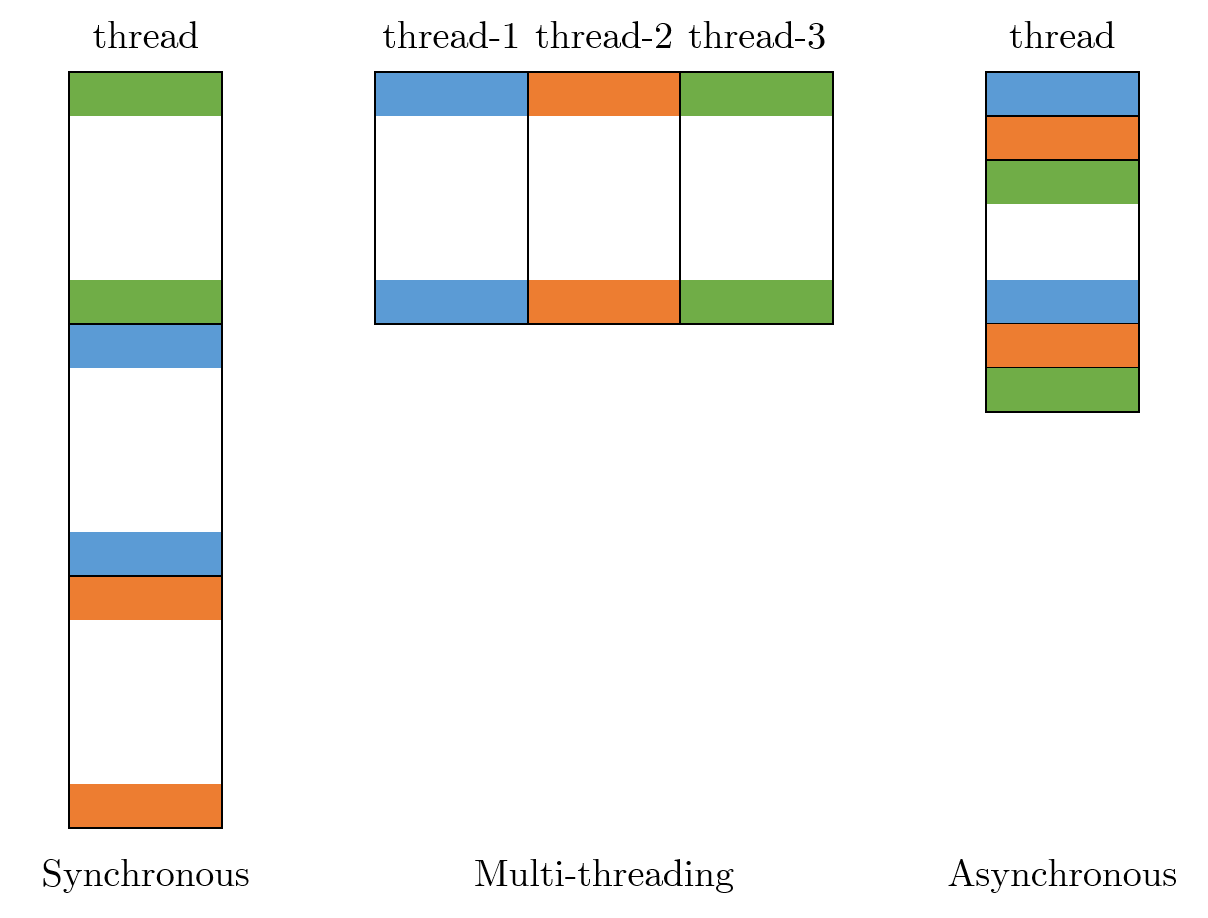
\includegraphics[width=4.5in]{fig/sma.png}
		\caption{Synchronous, Multi-threading and Asynchronous}
		\label{fig_sma}
	\end{figure}
	DBMS provides access by an open network port on operation system, the only entrance of interaction with the outside. For example, the default setting of MySQL assigns $3306$ as the number of service port. In the meanwhile, the client should connect to the port through Transmission Control Protocol (TCP) connection. Reminding the properties of TCP, a TCP connection, from its build-up to disconnection, includes three times of handshaking-connection and one notice of disconnection. 
	
	In simple programming tasks, we design the execution of programming statements naturally, which is synchronous. The synchronous method has its advantages that easy-reading code, low cost of finding bugs and insurance of the right order of events. However, its disadvantages are stick out when time-consuming events occur in the whole working flow. Time-consuming events, which are usually I/O operations due to the cost of communication with disk blocks and network hosts, block the working thread waiting for the returning result. In this period of time, CPUs are in idle and the computation resource is wasted. If, in most cases, there are multiple I/O operations, only one operation is done at a time. Contrary to the people waiting in the line boarding a flight, asynchronous I/O allows initiating multiple tasks and waiting for them simultaneously.
	
	Figure \ref{fig_sma} illustrates the diagram of synchronous programming, multi-threading and asynchronous programming. Tasks are labeled in different colors and the height of each colored box represents how long the thread is working on the event while white boxes are periods that the thread is waiting for the response. Asynchronous programming is not the same as multi-threading because it still has one thread activated rather than using more. Within the multi-threading, it remains the synchronous approach and the total waiting time hasn't been reduced, while it pays more system resources for us not waiting that long time in real world. 
	
	Asynchronous programming has its privileges on resource-time balancing. Coroutines are used in this situation to accomplish the task. Each coroutine is responsible for one or many asynchronous events as any other coroutines. The main thread can switch between coroutines on need when creating them, arranging tasks and gathering result. Compared to multi-threading, asynchronous programming has following outperformance:
	\begin{itemize}[\IEEEsetlabelwidth{Z}]
		\item Less system resources required when creating coroutines compared to sub-threadings. 
		\item Less cost on scheduling. Multi-threading entrust operation system (OS) to scheduling threads but coroutines need programmers' scheduling them manually. This leaves out unnecessary switching costs.
		\item Making the most of advantage of each the thread. Like I/O events, CPU idles when waiting for the response. Multi-threading occupies actual CPU threads and blocks other operations in corresponding threads. Coroutines are working on the single thread and one will be replaced by one of the others when comes to waiting. Thus, the waiting period occurs in synchronous programming will be covered by working period in asynchronous one.
	\end{itemize}
	
	\subsection{Our Work on Asynchronous DBMS Access}
	Considering DBMS access is a kind of time-consuming I/O operation, we apply asynchronous programming to organize DBMS access events, which is, from the coding perspective, to explore and implement methods of asynchronous DBMS access and pay attention to some important features. 
	
	Our work on this lab project mainly contains these contributions:
	\begin{itemize}
		\item Establish a database from an open-source dataset
		\item Implement a programme to access the DBMS asynchronously
		\item Design various kinds of experiments for observing performance indexes and future improvement.
	\end{itemize}
	
	Specifically, we are answering these questions:
	\begin{itemize}
		\item How to implement an asynchronous DBMS access in a specific program.
		\item Which kinds of SQL queries fit the asynchronous DBMS access.
		\item How much performance improvement gains from asynchronous DBMS access.
		\item What further modifications need for client and DBMS to adapt to asynchronous DBMS access.
	\end{itemize}
	
	\section{Working Environment}
	Our work is based on Python3 and MySQL5.7. The reason why we choose Python and MySQL is we are familiar with them. And Python supports the asynchronous programming which is feasible to perform the experiment. We select the video games part of Amazon review dataset as the source of data and use it to build an instance of the database containing several tables.
	
	\section{Asynchronous DBMS Access}
	First, to implement the asynchronous programming, we should know its mechanism and corresponding method in Python. 
	
	Python3 supports the asynchronous programming by a library, \textit{asyncio}~\cite{asyncio}, and keywords \textbf{async} and \textbf{await}. Keyword \textbf{async} is to define asynchronous functions and statements. In asynchronous function, keyword await is used to declare statements that will asynchronously execute. From the name \textbf{await}, it is also easy to comprehend that the statement before it will be hang up after being initiated and the thread will switch to execute other \textbf{await} statements ``waiting'' for running. Bringing time-consuming I/O operations into consideration, once an \textbf{await} statement is initiated and CPU seems to be idle in the following waiting period, CPU would execute other coroutines to prevent itself from being idle. Consequently, the CPU time is used with high efficiency. 
	
	Furthermore, outside the declaration of asynchronous function, an event loop is needed in the main thread. Library \textit{asyncio} provides an API for defining it, which is \textit{asyncio.get\_event\_loop()}. Generally, the only thing to do next is putting the asynchronous job into the loop and executing it by method \textit{loop.run\_until\_complete(task(params))}, where \textit{params} are parameters like any simple function. However, for multi-task situation, before we send the asynchronous events into the loop, we still need some work to arrange tasks for each coroutine. First, use \textit{asyncio.ensure\_future(task(params))} to create corresponding coroutines waiting for execution. Next, add each coroutine into a tasks list. Finally, use \textit{loop.run\_until\_complete(asyncio.wait(tasks))} to actually execute these coroutines.
	
	As for the part of DBMS connection, it should be placed in each coroutine. Here, we find a library called \textit{aiomysql} ~\cite{aiomysql}, which is based on \textit{aysncio} and \textit{pymysql}, providing simple API for asynchronously accessing the DBMS. Actually, there is no great difference between synchronous and asynchronous access in the form of exact coding. 
	
	Here we would like to present our basic framework accessing DBMS in Python code.
	\lstset{language=python,tabsize=2}
	\begin{lstlisting}
	async def exe_sql(item, lp):
	async with create_pool(host='localhost', port=3306,
	user='user', password='password',
	db='db', loop=lp) as pool:
	async with pool.get() as conn:
	async with conn.cursor() as cur:
	await cur.execute(''SQL Query'')
	await conn.commit()
	lp = asyncio.get_event_loop()
	tasks = [asyncio.ensure_future(exe_sql(item, lp)) for item in data]
	lp.run_until_complete(asyncio.wait(tasks))
	\end{lstlisting}
	
	By using Python3 codes above, the program has the ability to access the database asynchronously and save a large period of CPU time waiting for the result of queries. In next section, we are going to put forward our experiment methods and results, concerning on numbers about performance and analyzing what both programming and DBMS side should do to fit in the asynchronous access. 
	\section{Experiment}
	\subsection{Experiment Set Up}
	In addition to the working environment we illustrate above, we give our preparation on a dataset and building database. 
	We pick the part of video game review part of ~\cite{Amazon}, and we choose the version including only 5-core reviews from each reviewer, in order to keep our database in a suitable size. 
	
	From the original data, we import the .json file into MySQL database. They are constructed into two relational tables, the one is \textit{reviewer(\underline{reviewerID}, reviewerName)} and \textit{review(reviewerID, asin, helpful, reviewText, overall, summary, reviewTime, unixReviewTime)}. Note that because we are concentrated on conduct experiment for the purpose of asynchronous DBMS access, the content and the exact meaning of them are not essential. The importance lies in the size and relation, which means the probability to design some time-consuming SQL queries.
	
	\subsection{Inserting performance}
	
	\begin{figure}[!t]
		\centering
		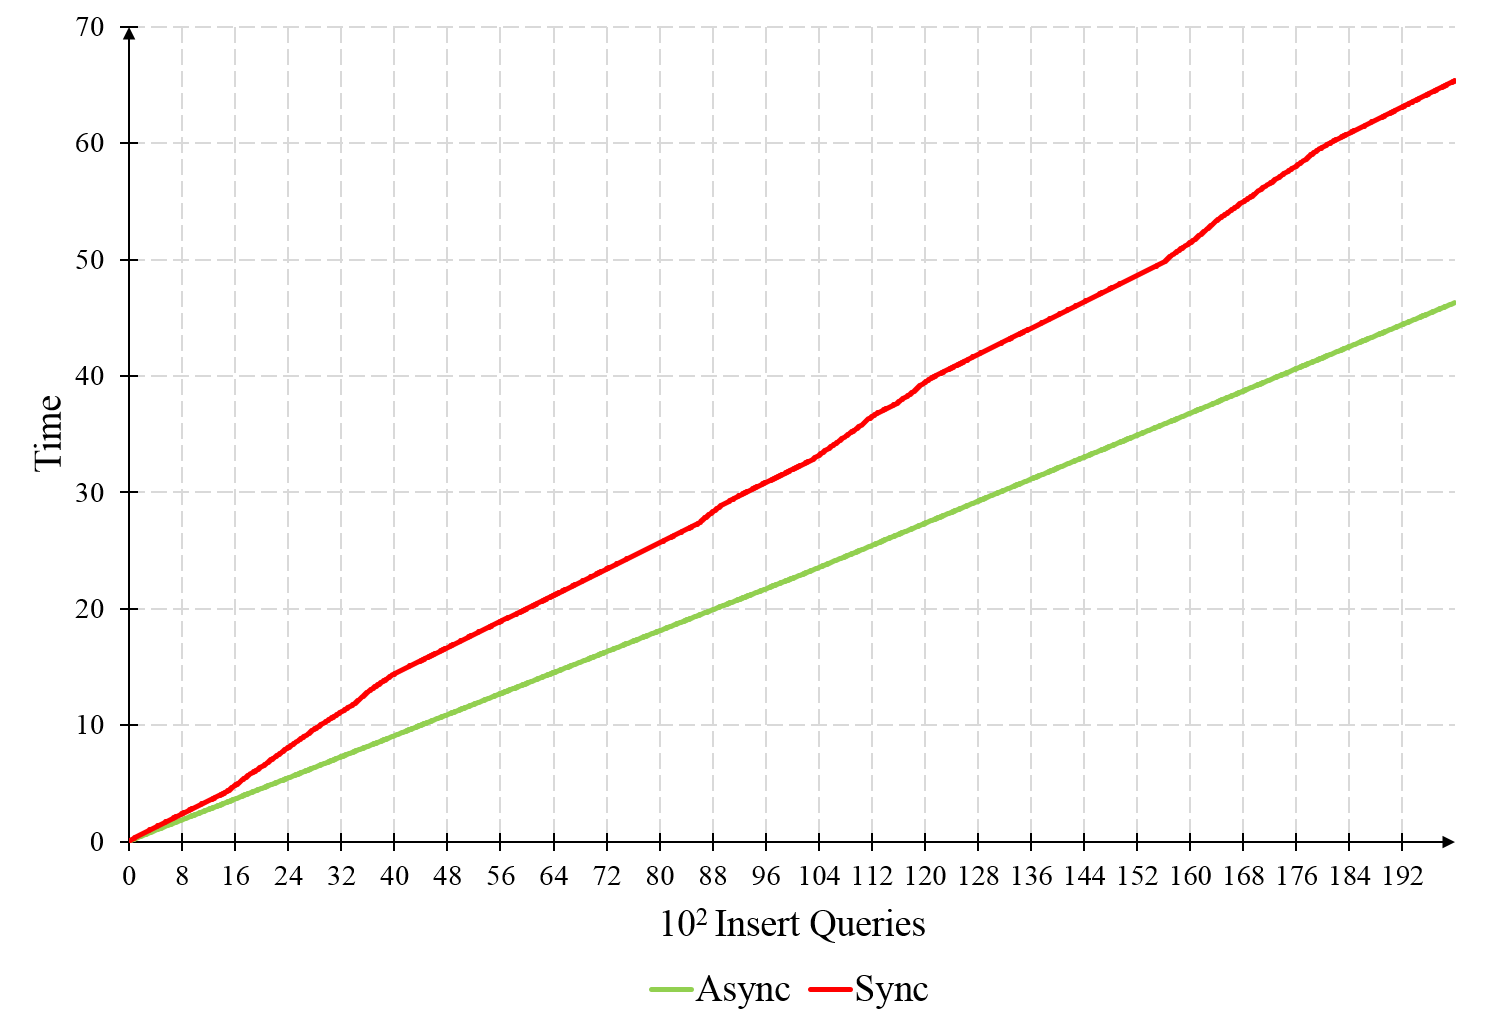
\includegraphics[width=6.5in]{fig/insert.png}
		\caption{Time Consumption of Insert}
		\label{fig_insert}
	\end{figure}
	Interestingly, we firstly implement the asynchronous access before we establish the database. Hence, we make use of this opportunity to insert data asynchronously using our program. In this attempt, we didn't limit the number of tasks and sent the queries continuously (about $ 220,000 $ queries) which run out of memory and cause the crash. Such amount of queries also were denied by the database. So we decreased the number of tasks and inserted the tuples. We also found that the CPU usage rate is about $ 5\% $ with synchronous access while $ 40\% $ with asynchronous access. 
	
	After that, we furthermore conduct the experiment with the more serious method. We insert $ 20000 $ tuples in a table with synchronous and asynchronous method respectively and record the consumption of time after inserting every 8 tuples. Figure \ref{fig_insert} shows the time consumption of two methods. Intuitively, asynchronous DBMS access can leverage the CPU computation resource more efficiently and save more time. The average speed of inserting with the asynchronous method is $ 432.06 $ tuples per second, which gains $ 41.18\% $ improvement as compared to the synchronous method with the average speed $ 306.04 $ tuples per second. Also, it’s obvious that the speed of asynchronous DBMS access is stable.
	
	\subsection{Performance Improvement and Limitation on Select Operation}
	Option \textbf{Select} may be the most common one of database access in the real world, so it is worth to investigate how much performance improvement gain with asynchronous database access. Thus, the experiment simulates a mount of access with \textbf{Select} in synchronous and asynchronous way respectively and records the time consuming. To explore the influence and limitation of asynchronous tasks, we design experiments about different number of tasks in asynchronous access. To avoid the performance influence of database cache, the queries are generated randomly to request for different tuples. 
	
	\begin{figure}[!t]
		\centering
		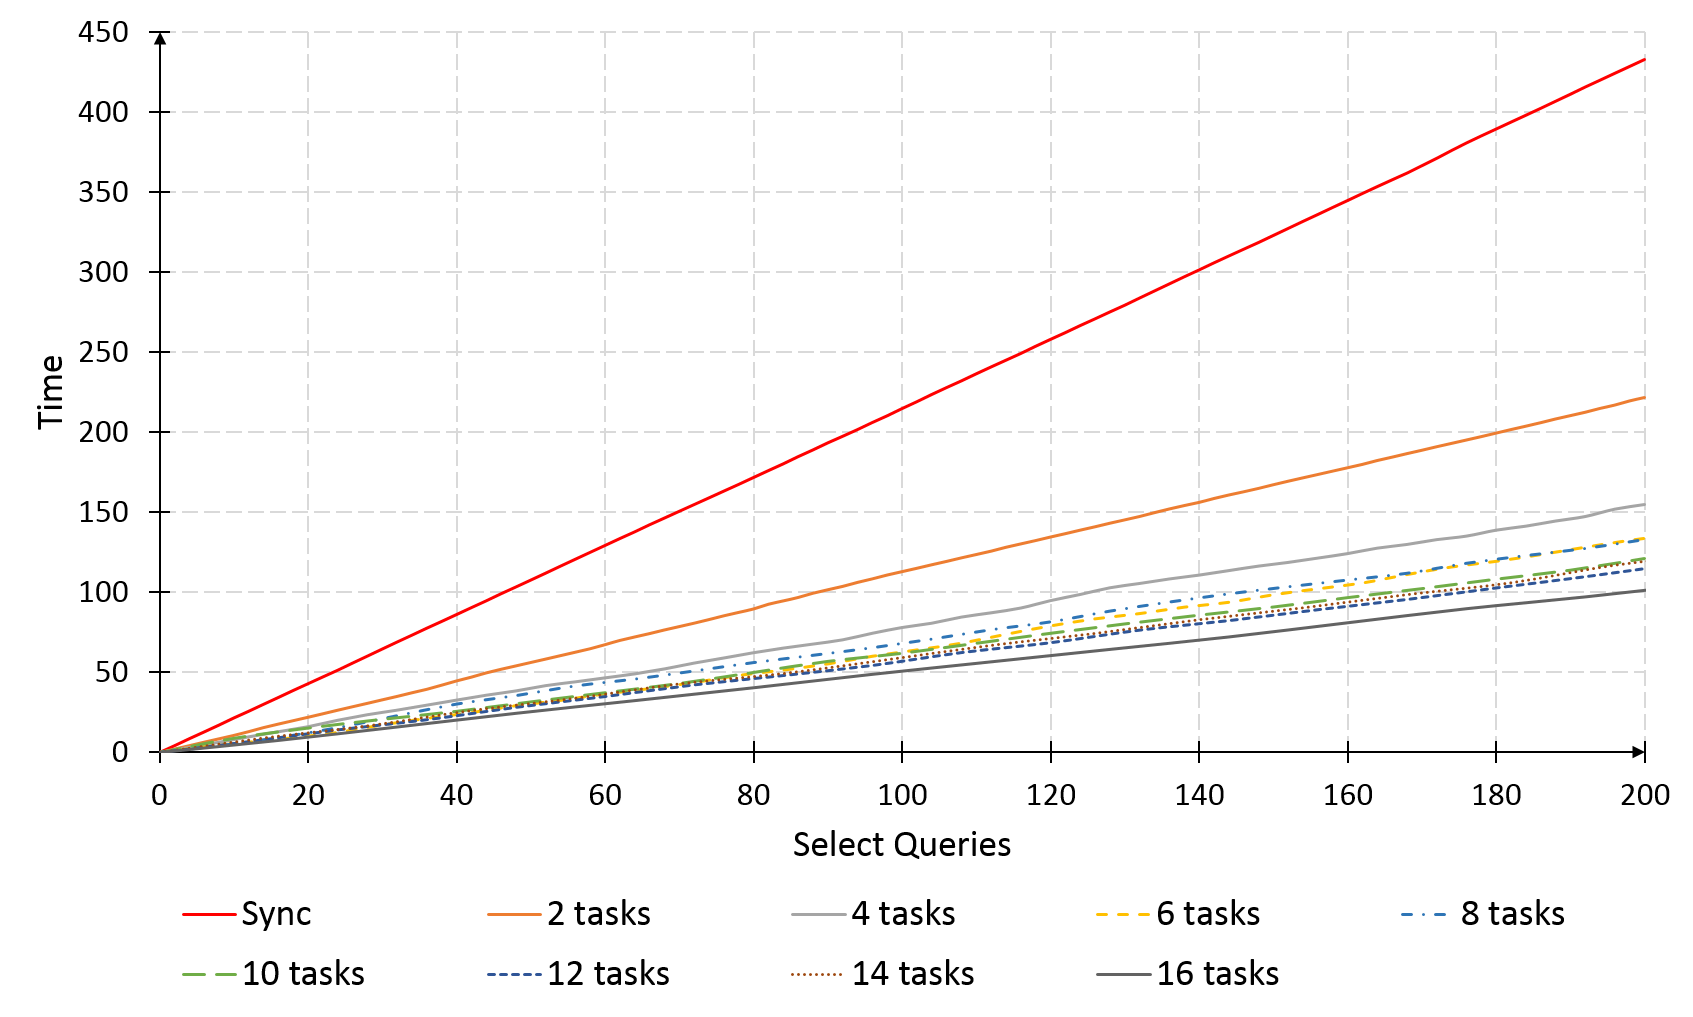
\includegraphics[width=6.5in]{fig/select.png}
		\caption{Time Consumption of Select with Different Number of Tasks}
		\label{fig_select}
	\end{figure}
	
	Figure \ref{fig_select} shows the time consuming of synchronous access and asynchronous access with different tasks. It can be drawn that the asynchronous access can bring performance improvement gain. And with the increased number of tasks, the performance also increases but its pace is getting slower. Maybe for \textbf{Select} option, 8 tasks could occupy all the waiting time so that the performance won't increase after that. 
	
	\begin{table}
		\centering
		\caption{Time Consumption of \textbf{Select} with Different Condition}
		\begin{tabular}{|c|c|c|c|c|}
			\hline
			Sync/Async & Queries & Tasks & Returned Tuples & Time\\
			\hline
			Synchronous & 200 & / & 3338732	& 432.4\\
			\hline
			Asynchronous & 200 & 2 & 3138212 & 221.4\\
			\hline
			Asynchronous & 200 & 4 & 3059651 & 154.6\\
			\hline
			Asynchronous & 204 & 6 & 3523492 & 135.8\\
			\hline
			Asynchronous & 200 & 8 & 2976721 & 132.5\\
			\hline
			Asynchronous & 200 & 10 & 3127633 & 121.1\\
			\hline
			Asynchronous & 204 & 12 & 3382936 & 117.2\\
			\hline
			Asynchronous & 210 & 14 & 3491832 & 123.9\\
			\hline
			Asynchronous & 208 & 16 & 3271681 & 105.2\\
			\hline
		\end{tabular}
		\label{T1}
	\end{table}
	
	Since random queries may fetch different number of tuples which may be related to the performance, we also statistic the number of them and show them on Table I. Also the concrete number of tasks, queries and time consuming are shown on the table. 
	
	\subsection{Updating Performance}
	It is interesting about what is shown on Fig.4 that it costs more on \emph{UPDATE} option of asynchronous access compare to synchronous. The reason may be that the database lock the table when executing \emph{UPDATE} and the next query should wait for it. And because of the connection cost the performance decreases with asynchronous access. 
	   
	
	
	\subsection{Impact of different database operations}
	
	There are many different database operations. Asynchronous DBMS access may not fit everyone. In addition to \textbf{Insert}, we investigate other four typical operations, including \textbf{Select}, \textbf{Join}, \textbf{Count}, and \textbf{Update}. Table \ref{T1} shows the time consumption of these operations synchronously and asynchronously with $ 40 $ tasks. Table \ref{T2} shows the average speed of them. The performance improvement of different operations varies greatly. Selecting data and joining tables gain $ 185.7\% $ and $ 154.4\% $ improvement respectively, while aggregate functions \textbf{Count} with asynchronous method outperform synchronous access with a great improvement of $ 1181.6\% $. Obviously, asynchronous DBMS access has strong capability to manage aggregate functions. However, as shown in Figure \ref{fig_update}, it is interesting that when we update data asynchronously, we even cost more time than synchronous method. Maybe this kind of SQL queries do not fit the asynchronous DBMS access.
	
	\begin{table}
		\centering
		\caption{Time Consumption of Typical Operations}
		\begin{tabular}{|c|c|c|c|c|c|}
			\hline
			& Insert & Select & Join & Count & Update\\
			\hline
			synchronous & 158.3 & 86.08 & 1220 & 664.4 & 84.57\\
			\hline
			asynchronous & 116.1 & 30.13 & 479.6 & 51.84 & 85.43\\
			\hline
		\end{tabular}
		\label{T1}
	\end{table}
	
	\begin{table}
		\centering
		\caption{Average Speed of Typical Operations}
		\begin{tabular}{|c|c|c|c|c|c|}
			\hline
			& Insert & Select & Join & Count & Update\\
			\hline
			synchronous & 0.2527 & 0.4647 & 0.0328 & 0.0602 & 0.4730\\
			\hline
			asynchronous & 0.3445 & 1.3276 & 0.0834 & 0.7716 & 0.4682\\
			\hline
		\end{tabular}
		\label{T2}
	\end{table}
	
	\begin{figure}[!t]
		\centering
		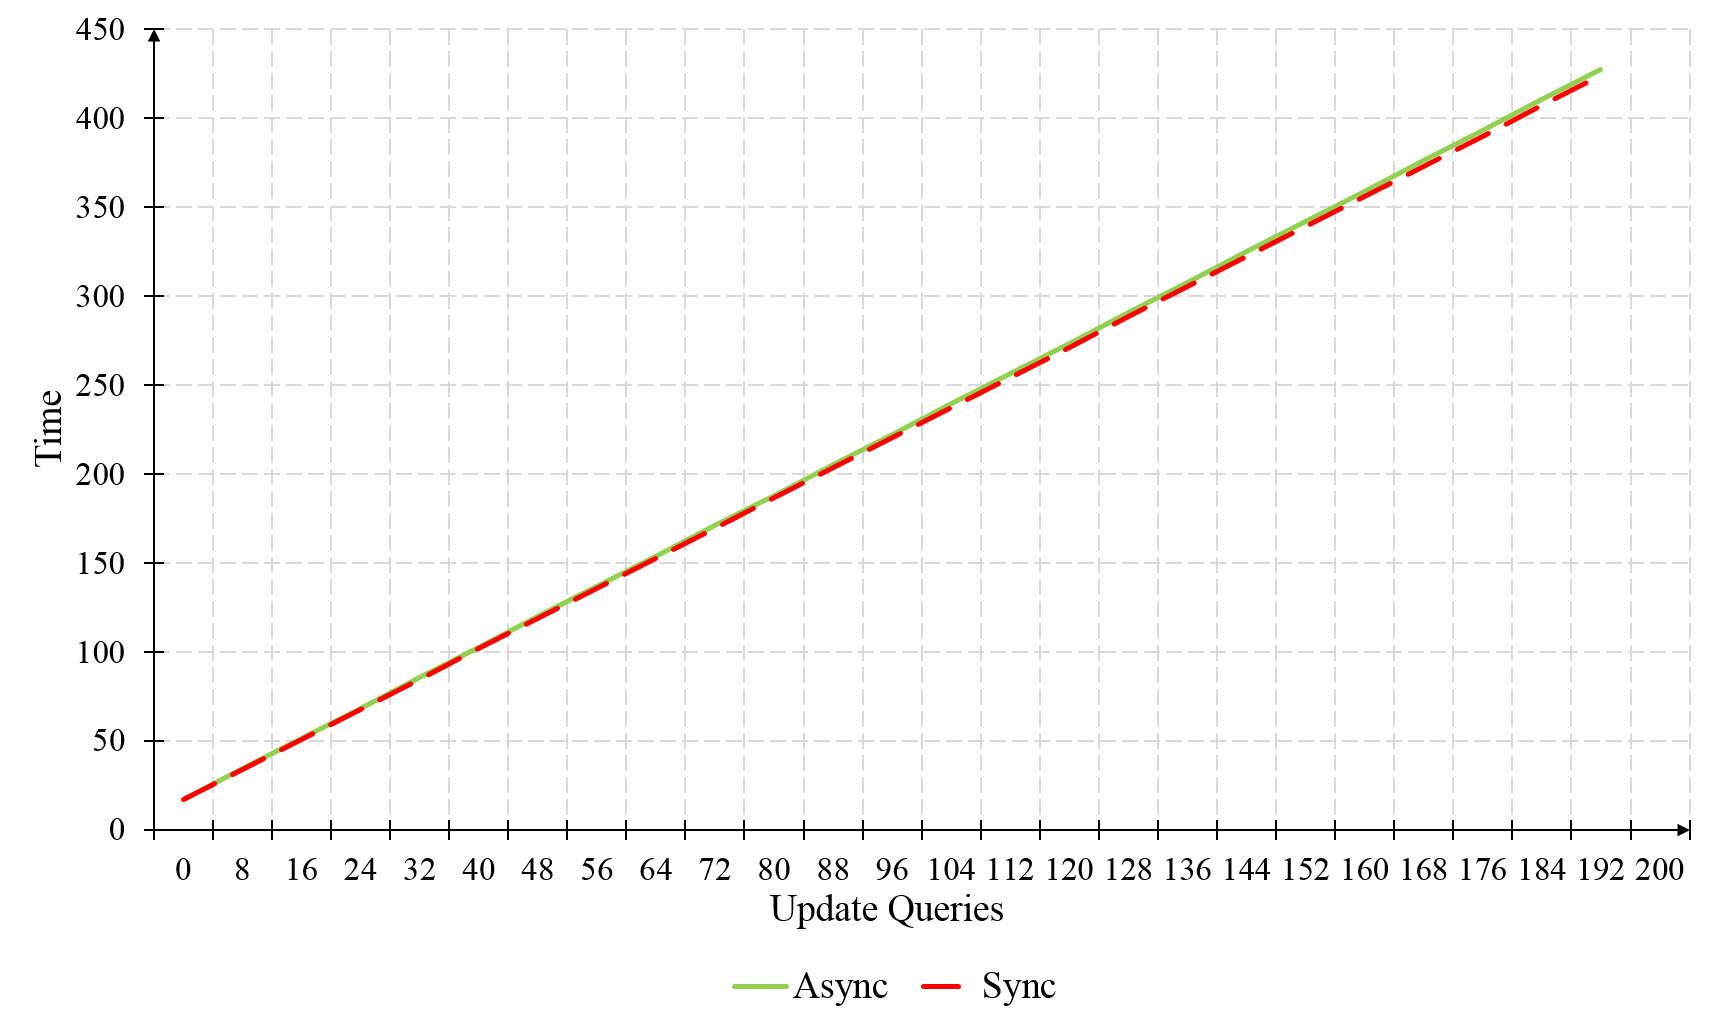
\includegraphics[width=6.5in]{fig/update.png}
		\caption{Time Consumption of Update}
		\label{fig_update}
	\end{figure}
	\section{Conclusion}

	From all of experiments above, we are able to uncover several problems related to asynchronous DBMS access:
	\begin{itemize}
		\item CPU and other computational resource overwhelming on a client when initiating large amount of coroutines.
		\item Limitation in maximum TCP connections established on both a client and a DBMS. A large number of asynchronous from one thread at the same time causes some of queries are missing and ignored, even failed to establish TCP connection.
		\item Queries jam in DBMS. Similar to the previous point, this also slows down the execution efficiency and drops out some equeries.
		\item Query scheduling. How to arrange the order of query execution in the DBMS.
		\item Database security. Due to the potential high frequency of sending queries, a DBMS system my be attacted by this method. 
	\end{itemize}
	
	Aiming at these proposed problems, we, to the best of our knowledge, present following potential modifications applied on DBMS to address them:
	\begin{itemize}
		\item Enlarge the network capacity of a DBMS to insure the quantity and efficiency TCP connections.
		\item Insure that DBMS supports multi-threading in executing queries. Ideally, one coroutine from a client corresonds one or more threads running DBMS for the alrgest working efficiency. Otherwise, single thread in DBMS will not develop the ability of asynchronous access, which acutually still remains synchronously single thread.
		\item Apply advanced scheduling algorithms in DBMS in cooperation with asynchronous DBMS access from clien to reduce overall waiting time, even including predicting execution time of a query for better scheduling.
		\item Optimize \textbf{Read} and \textbf{Write} locks when updating a table. We learn that there exists a technology that only locking the related part of the table when performing updates, while other unrelated transactions are not blocked.
		\item Intelligent detection of malicious access. 
	\end{itemize}
	
	To sum up, in this project, we establish a database from an open-source dataset, and implement a program to access the DBMS asynchronously. Then, we design various kinds of experiments for observing the performance improvement of asynchronous method. We show that A non-blocking interface allowing a single client thread to issue many parallel queries from the same thread brings us impressive performance gains. Except \textbf{Update}, every kind of SQL queries with asynchronous method outperform synchronous access with a huge improvement efficiency. As for aggregate functions, the improvement is even up to $ 1181.6\% $. Finally, we conclude some problems observed from out experiments and present possible solutions to address the problem.
	
	
	% An example of a floating figure using the graphicx package.
	% Note that \label must occur AFTER (or within) \caption.
	% For figures, \caption should occur after the \includegraphics.
	% Note that IEEEtran v1.7 and later has special internal code that
	% is designed to preserve the operation of \label within \caption
	% even when the captionsoff option is in effect. However, because
	% of issues like this, it may be the safest practice to put all your
	% \label just after \caption rather than within \caption{}.
	%
	% Reminder: the "draftcls" or "draftclsnofoot", not "draft", class
	% option should be used if it is desired that the figures are to be
	% displayed while in draft mode.
	%
	%\begin{figure}[!t]
	%\centering
	%\includegraphics[width=2.5in]{myfigure}
	% where an .eps filename suffix will be assumed under latex, 
	% and a .pdf suffix will be assumed for pdflatex; or what has been declared
	% via \DeclareGraphicsExtensions.
	%\caption{Simulation results for the network.}
	%\label{fig_sim}
	%\end{figure}
	
	% Note that the IEEE typically puts floats only at the top, even when this
	% results in a large percentage of a column being occupied by floats.
	
	
	% An example of a double column floating figure using two subfigures.
	% (The subfig.sty package must be loaded for this to work.)
	% The subfigure \label commands are set within each subfloat command,
	% and the \label for the overall figure must come after \caption.
	% \hfil is used as a separator to get equal spacing.
	% Watch out that the combined width of all the subfigures on a 
	% line do not exceed the text width or a line break will occur.
	%
	%\begin{figure*}[!t]
	%\centering
	%\subfloat[Case I]{\includegraphics[width=2.5in]{box}%
	%\label{fig_first_case}}
	%\hfil
	%\subfloat[Case II]{\includegraphics[width=2.5in]{box}%
	%\label{fig_second_case}}
	%\caption{Simulation results for the network.}
	%\label{fig_sim}
	%\end{figure*}
	%
	% Note that often IEEE papers with subfigures do not employ subfigure
	% captions (using the optional argument to \subfloat[]), but instead will
	% reference/describe all of them (a), (b), etc., within the main caption.
	% Be aware that for subfig.sty to generate the (a), (b), etc., subfigure
	% labels, the optional argument to \subfloat must be present. If a
	% subcaption is not desired, just leave its contents blank,
	% e.g., \subfloat[].
	
	
	% An example of a floating table. Note that, for IEEE style tables, the
	% \caption command should come BEFORE the table and, given that table
	% captions serve much like titles, are usually capitalized except for words
	% such as a, an, and, as, at, but, by, for, in, nor, of, on, or, the, to
	% and up, which are usually not capitalized unless they are the first or
	% last word of the caption. Table text will default to \footnotesize as
	% the IEEE normally uses this smaller font for tables.
	% The \label must come after \caption as always.
	%
	%\begin{table}[!t]
	%% increase table row spacing, adjust to taste
	%\renewcommand{\arraystretch}{1.3}
	% if using array.sty, it might be a good idea to tweak the value of
	% \extrarowheight as needed to properly center the text within the cells
	%\caption{An Example of a Table}
	%\label{table_example}
	%\centering
	%% Some packages, such as MDW tools, offer better commands for making tables
	%% than the plain LaTeX2e tabular which is used here.
	%\begin{tabular}{|c||c|}
	%\hline
	%One & Two\\
	%\hline
	%Three & Four\\
	%\hline
	%\end{tabular}
	%\end{table}
	
	
	% Note that the IEEE does not put floats in the very first column
	% - or typically anywhere on the first page for that matter. Also,
	% in-text middle ("here") positioning is typically not used, but it
	% is allowed and encouraged for Computer Society conferences (but
	% not Computer Society journals). Most IEEE journals/conferences use
	% top floats exclusively. 
	% Note that, LaTeX2e, unlike IEEE journals/conferences, places
	% footnotes above bottom floats. This can be corrected via the
	% \fnbelowfloat command of the stfloats package.
	
	
	
	
	
	
	
	
	
	% conference papers do not normally have an appendix
	
	
	% use section* for acknowledgment
	
	% trigger a \newpage just before the given reference
	% number - used to balance the columns on the last page
	% adjust value as needed - may need to be readjusted if
	% the document is modified later
	%\IEEEtriggeratref{8}
	% The "triggered" command can be changed if desired:
	%\IEEEtriggercmd{\enlargethispage{-5in}}
	
	% references section
	
	% can use a bibliography generated by BibTeX as a .bbl file
	% BibTeX documentation can be easily obtained at:
	% http://mirror.ctan.org/biblio/bibtex/contrib/doc/
	% The IEEEtran BibTeX style support page is at:
	% http://www.michaelshell.org/tex/ieeetran/bibtex/
	\bibliographystyle{IEEEtran}
	% argument is your BibTeX string definitions and bibliography database(s)
	\bibliography{async}
	%
	% <OR> manually copy in the resultant .bbl file
	% set second argument of \begin to the number of references
	% (used to reserve space for the reference number labels box)
	% \begin{thebibliography}{1}
	
	%     \bibitem{IEEEhowto:kopka}
	%     H.~Kopka and P.~W. Daly, \emph{A Guide to \LaTeX}, 3rd~ed.\hskip 1em plus
	%     0.5em minus 0.4em\relax Harlow, England: Addison-Wesley, 1999.
	
	% \end{thebibliography}
	
	
	
	
	% that's all folks
\end{document}











